\chapter{Grid techniques used in this thesis}
\label{Grid}

The following section provides a summary of the Grid environment facilities used in this thesis work.

\begin{figure}[ht]
\centering
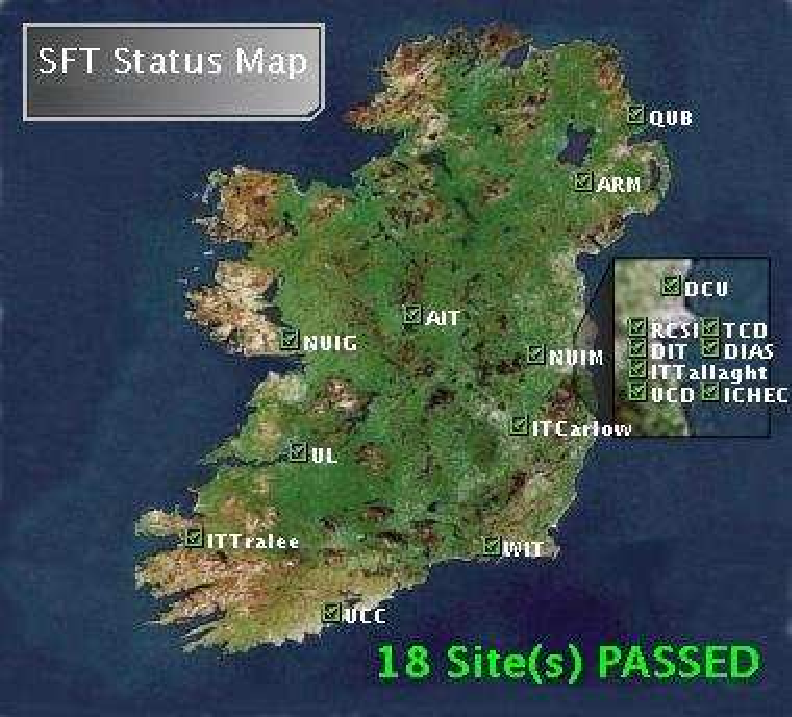
\includegraphics[width=8cm]{GridIreland}
\caption{
Grid Ireland sites
}
\label{fig:Grid} % label
\end{figure}




The future of scientific computing may well lie in the use of grid technology to link together sparse resources into a large-scaled loosely-coupled distributed computing facility. Such systems are already in place, including for example the Grid-Ireland system, which in this research has been harnessed to calculate the distribution of extincting dust in the galactic plane, and in various star-forming regions.




The Grid interface consists of a single sign-on authentication using a grid certificate, followed by submission of jobs to the grid middleware, for distribution around the grid computing elements (CEs). Data may be stored on storage elements (SEs), or very small amounts of data ( $\sim$ 2 MB ) may be submitted from the grid gateway using the input sandbox.


\section{Single-sign-on Authentication}
In the course of this thesis work - ten systems were used all with various different userids, passwords and public key infrastructure identities, compilers, libraries and architectures. 
The Grid single-sign on authentication offers the opportunity to access all systems linked to the Grid without requiring a user account and password on each system.
Access is obtained using a digital certificate which is downloaded from the Grid-Ireland website.
The grid certificate is then copied to a gateway machine, which is the only machine on which a userid is required.
The certificate is actually used via a proxy, which has a specified lifetime defaulting to 24 hours and with a maximum of one week.
%The default lifetime of 24 hours was too short for the extinction mapping.
Both the default and maximum proxy lifetimes were too short so the job was further subdivided into 4 manageable chunks.
%It also offers a single gateway to different and geographically separate locations.

\section{Data storage and retrieval}
Data may be stored at arbitrarily on the Grid and retrieved at a later stage. 
There are several tools for doing this (e.g. grid-ftp, globus-url-copy and lcg-cp).
The lcg (Large Hadron Collider Computational Grid) suite was used to copy data and programs about the grid.
Example:
\textcolor{green}
{\textsf {
lcg-cr --vo CosmoGrid file:ext.tar  -l lfn:extfiles.tar -d gridstore.cs.tcd.ie
}}
In the work done in this thesis the time taken to access to Grid storage facilities represented a significant portion of the entire wall clock time, and it was initially thought quicker to send the data using the Input Sandbox.
However this proved somewhat shortsighted as the number of jobs was significantly increased (to 8,000); the Input Sandbox technique slowed down the submission and caused jobs to fail.
This problem was addressed by resubmitting the jobs - ultimately the grid copy strategy was the correct one.


\section{Job Submission}

%The batch submission technique in the heterogeneous grid environment is different as resources in different locations can be requested.

As the Grid is a heterogeneous environment, if specific resources (e.g. compilers, accessible storage, specific architecture, message-passing abilities, shared memory etc.) are required, they must be specified using the Job Submission Description Language.
To illustrate this, some examples are shown.
%A specified desired software runtime environment may be requested using 
Ray-tracing software may be requested using the command
\textcolor{green}
{\textsf {
\\Requirements = 
\\Member("POVRAY-3.1",other.GlueHostApplicationSoftwareRunTimeEnvironment);
}}
\\A specified operating system may be requested using the command
\textcolor{green}
{\textsf {
\\Requirements = other.GlueHostOperatingSystemName == "Redhat";
}}
\\To use parallel environments, it was necessary to specify the number of nodes
\textcolor{green}
{\textsf {
\\JobType= "MPICH"
\\NodeNumber = 8
}}

